
\documentclass{article}
\usepackage{graphicx}
\usepackage{hyperref}
\usepackage{amsmath,natbib}
\usepackage{times,verbatim}

\textwidth=6.2in
\textheight=8.5in
%\parskip=.3cm
\oddsidemargin=.1in
\evensidemargin=.1in
\headheight=-.3in


%------------------------------------------------------------
% newcommand
%------------------------------------------------------------
\newcommand{\scscst}{\scriptscriptstyle}
\newcommand{\scst}{\scriptstyle}
\newcommand{\Robject}[1]{{\texttt{#1}}}
\newcommand{\Rfunction}[1]{{\texttt{#1}}}
\newcommand{\Rclass}[1]{\textit{#1}}
\newcommand{\Rpackage}[1]{\textit{#1}}
\newcommand{\Rexpression}[1]{\texttt{#1}}
\newcommand{\Rmethod}[1]{{\texttt{#1}}}
\newcommand{\Rfunarg}[1]{{\texttt{#1}}}

\usepackage{Sweave}
\begin{document}
\Sconcordance{concordance:manual.tex:manual.Rnw:%
1 28 1 1 0 20 1 1 2 1 0 1 1 3 0 1 2 6 1 1 2 6 0 1 1 22 0 1 1 5 0 1 1 6 %
0 1 2 2 1 1 2 1 0 14 1 3 0 1 2 2 1 1 2 1 0 1 1 18 0 1 1 5 0 1 1 5 0 1 1 %
5 0 1 1 5 0 1 1 5 0 1 1 6 0 1 2 7 1 1 6 12 0 1 2 7 1 1 2 14 0 1 2 1 1 1 %
2 1 0 1 1 6 0 1 2 1 1 1 2 8 0 1 2 2 1 1 2 64 0 1 2 1 1 1 2 8 0 2 1 6 0 %
1 2 2 1 1 2 9 0 1 2 1 1 1 2 6 0 1 1 6 0 1 2 8 1 1 2 7 0 1 1 11 0 1 1 6 %
0 1 2 10 1 1 2 4 0 1 2 12 1 1 2 4 0 1 2 2 1 1 2 4 0 1 2 2 1 1 6 11 0 1 %
1 6 0 1 1 11 0 1 1 5 0 1 1 3 0 2 2 4 0 1 2 4 1 1 2 1 0 1 1 1 6 5 0 1 2 %
5 0 1 2 2 1 1 3 2 0 1 1 1 3 1 0 1 1 1 3 1 0 1 1 1 2 2 1 1 2 1 22 20 0 1 %
2 1 17 15 0 1 2 1 1 1 7 5 0 1 2 1 0 1 3 1 0 2 1 4 0 1 2 1 1 1 2 1 0 1 5 %
10 0 1 1 6 0 1 1 11 0 1 1 5 0 1 1 3 0 1 2 1 1 1 2 1 0 1 1 1 2 1 17 15 0 %
1 3 6 0 1 3 5 1 1 2 35 0 1 2 4 1}


%------------------------------------------------------------
\title{PReMiuM manual}
%------------------------------------------------------------
\author{Silvia Liverani}
%\date{}





\maketitle
\tableofcontents

%-------------------------------------------
\section{Introduction}
%--------------------------------------------
First of all, we load the R package PReMiuM and set a seed to ensure every run gives the same results in this manual. 

\begin{Schunk}
\begin{Sinput}
> library(PReMiuM)
> set.seed(1234)
\end{Sinput}
\end{Schunk}

%-------------------------------------------
\section{Generating data}
%--------------------------------------------

PReMiuM includes a few functions to generate data. The data is generated by the function generateSampleDataFile(). The input of the function is a list of parameters. In the example below we generated a Bernoulli (ie. binary) distributed outcome and discrete covariates. The exact parameters of the data generating functions are obtained by writing the command in R. Some of the values returned in a list by this function are shown below: cluster sizes; the parameters for cluster 1 (value of $\theta_1$ as well as the probabilities for the categories of the 5 discrete covariates - they all 3 levels); the vector of fixed effect coefficients $\beta$ and the probability with which missing values are to be inputted into the dataset.

\begin{Schunk}
\begin{Sinput}
> clusSummaryBernoulliDiscrete()$clusterSizes
\end{Sinput}
\begin{Soutput}
[1] 200 200 200 200 200
\end{Soutput}
\begin{Sinput}
> clusSummaryBernoulliDiscrete()$clusterData[[1]]
\end{Sinput}
\begin{Soutput}
$theta
[1] 2.197225

$covariateProbs
$covariateProbs[[1]]
[1] 0.8 0.1 0.1

$covariateProbs[[2]]
[1] 0.8 0.1 0.1

$covariateProbs[[3]]
[1] 0.8 0.1 0.1

$covariateProbs[[4]]
[1] 0.8 0.1 0.1

$covariateProbs[[5]]
[1] 0.8 0.1 0.1
\end{Soutput}
\begin{Sinput}
> clusSummaryBernoulliDiscrete()$fixedEffectsCoeffs
\end{Sinput}
\begin{Soutput}
[1]  0.1 -0.5
\end{Soutput}
\begin{Sinput}
> clusSummaryBernoulliDiscrete()$missingDataProb
\end{Sinput}
\begin{Soutput}
[1] 0
\end{Soutput}
\end{Schunk}

Other functions to generate data from other models (the names of the functions should be self explanatory). 

\begin{Schunk}
\begin{Sinput}
> clusSummaryBernoulliDiscrete()
> clusSummaryBernoulliNormal
> clusSummaryBernoulliDiscreteSmall()
> clusSummaryBinomialNormal()
> clusSummaryCategoricalDiscrete()
> clusSummaryNormalDiscrete()
> clusSummaryNormalNormal()
> clusSummaryNormalNormalSpatial()
> clusSummaryPoissonDiscrete()
> clusSummaryPoissonNormal()
> clusSummaryPoissonNormalSpatial()
> clusSummaryVarSelectBernoulliDiscrete()
> clusSummaryBernoulliMixed()
> clusSummaryWeibullDiscrete()
> clusSummaryQuantileNormal()
\end{Sinput}
\end{Schunk}

The data is then generated as follows. The dataset is stored in a list environment with the following output obtained when running it. 

\begin{Schunk}
\begin{Sinput}
> inputs <- generateSampleDataFile(clusSummaryBernoulliDiscrete())
> head(inputs$inputData)
\end{Sinput}
\begin{Soutput}
  outcome Variable1 Variable2 Variable3 Variable4 Variable5 FixedEffects1
1       1         0         0         0         0         1   -0.61197199
2       1         0         0         0         0         0    0.17096033
3       1         0         0         0         0         0    2.32525273
4       1         0         1         0         0         0   -0.03949958
5       1         0         2         0         0         0    1.74155924
6       1         0         0         0         0         0   -0.55800892
  FixedEffects2
1   -0.44617094
2   -0.82669610
3   -1.12031150
4    0.05577411
5    1.21821120
6    1.14820273
\end{Soutput}
\begin{Sinput}
> inputs$covNames
\end{Sinput}
\begin{Soutput}
[1] "Variable1" "Variable2" "Variable3" "Variable4" "Variable5"
\end{Soutput}
\begin{Sinput}
> inputs$xModel
\end{Sinput}
\begin{Soutput}
[1] "Discrete"
\end{Soutput}
\begin{Sinput}
> inputs$yModel
\end{Sinput}
\begin{Soutput}
[1] "Bernoulli"
\end{Soutput}
\begin{Sinput}
> inputs$nCovariates
\end{Sinput}
\begin{Soutput}
[1] 5
\end{Soutput}
\begin{Sinput}
> inputs$fixedEffectNames
\end{Sinput}
\begin{Soutput}
[1] "FixedEffects1" "FixedEffects2"
\end{Soutput}
\begin{Sinput}
> inputs$outcomeT
\end{Sinput}
\begin{Soutput}
NULL
\end{Soutput}
\end{Schunk}

%-------------------------------------------
\section{Running PReMiuM}
%--------------------------------------------
We can now run profile regression using the data simulated above. The command profRegr(), which runs profile regression, is effectively running an MCMC. For that reason, it is recommended that it runs over many thousands, or tens of thousands, or more iterations. However, for simplicity and speed we will only run the MCMC for very few iterations in this manual. The burn in period is determined by the option nBurn and the number of iterations following the burn-in period is determined by the option nSweeps. 

The output of this function is very large, so it is all saved in external files which are created when the command is run. For this reason it is important to know in which folder the command is to be run, to know where to find the output files. The files will all be named \verb|xyz_content.txt| where \verb|xyz| is the name of the profile regression run and can be set by providing option output (which in the example below is \verb|output|) and \verb|content| is the content of the file (explained in more detail in the following section).

\begin{Schunk}
\begin{Sinput}
> runInfoObj<-profRegr(yModel=inputs$yModel, 
+     xModel=inputs$xModel, nSweeps=100, nClusInit=15,
+     nBurn=300, data=inputs$inputData, output="output", 
+     covNames = inputs$covNames, 
+     fixedEffectsNames = inputs$fixedEffectNames, seed=12345)
\end{Sinput}
\begin{Soutput}
Random number seed: 12345
Sweep: 1
\end{Soutput}
\end{Schunk}

%-------------------------------------------
\subsection{Outputs of profRegr()}
%--------------------------------------------
Several files are created when \verb|profRegr()| is run. We discuss the most important files below. 

\begin{description}
\item[Data input] Before running the MCMC, profRegr() reads the inputs file and creates a file with the information needed to run the MCMC. The first 10 lines of this file are printed below. 
\begin{Schunk}
\begin{Sinput}
> readLines("output_input.txt",15)
\end{Sinput}
\begin{Soutput}
 [1] "1000"                               "5"                                 
 [3] "Variable1"                          "Variable2"                         
 [5] "Variable3"                          "Variable4"                         
 [7] "Variable5"                          "2"                                 
 [9] "FixedEffects1"                      "FixedEffects2"                     
[11] "3 3 3 3 3"                          "1 0 0 0 0 1 -0.611972 -0.4461709"  
[13] "1 0 0 0 0 0 0.1709603 -0.8266961"   "1 0 0 0 0 0 2.325253 -1.120312"    
[15] "1 0 1 0 0 0 -0.03949958 0.05577411"
\end{Soutput}
\end{Schunk}

\item[Number of clusters] This file is of length equal to nSweeps (the number of iterations of the MCMC after the burn in period). Each line corresponds to an iteration and it includes a signle number, which is the number of clusters in that iteration. 
\begin{Schunk}
\begin{Sinput}
> nClustersSweep1<-read.table("output_nClusters.txt")[1,1]
> nClustersSweep1
\end{Sinput}
\begin{Soutput}
[1] 15
\end{Soutput}
\end{Schunk}

\item[Number of observations in each cluster] Each line of this file corresponds to one iteration of the MCMC. Each line gives the size of the clusters. The last number is the total number of observations clustered (ie the sum of all preceeding numbers in the line). The first line of this file is shown below.  
\begin{Schunk}
\begin{Sinput}
> as.numeric(strsplit(readLines("output_nMembers.txt",1)," ")[[1]])
\end{Sinput}
\begin{Soutput}
 [1]   49  201  213   10    2  186    9  178  140   10    1    0    1    0    0
[16] 1000
\end{Soutput}
\end{Schunk}

\item[Log] This file includes several details about the MCMC run, including the parameters used, the MCMC samplers used, their acceptance rate, etc. See below. 

\begin{Schunk}
\begin{Sinput}
> readLines("output_log.txt")
\end{Sinput}
\begin{Soutput}
 [1] "Date and time: 2017-06-19 12:0917"                                         
 [2] ""                                                                          
 [3] "Data file path: output_input.txt"                                          
 [4] ""                                                                          
 [5] "Output file path: output"                                                  
 [6] ""                                                                          
 [7] "Predict file path: No predictions run."                                    
 [8] ""                                                                          
 [9] "Seed: 12345"                                                               
[10] ""                                                                          
[11] "Number of sweeps: 100"                                                     
[12] "Burn in sweeps: 300"                                                       
[13] "Output filter: 1"                                                          
[14] "Proposal Type: gibbsForVActive, Acceptance Rate: 1"                        
[15] "Proposal Type: updateForPhiActive, Acceptance Rate: 1"                     
[16] "Proposal Type: metropolisHastingsForThetaActive, Acceptance Rate: 0.438538"
[17] "Proposal Type: metropolisHastingsForBeta, Acceptance Rate: 0.37875"        
[18] "Proposal Type: gibbsForU, Acceptance Rate: 1"                              
[19] "Proposal Type: metropolisHastingsForAlpha, Acceptance Rate: 0.4175"        
[20] "Proposal Type: gibbsForVInActive, Acceptance Rate: 1"                      
[21] "Proposal Type: gibbsForPhiInActive, Acceptance Rate: 1"                    
[22] "Proposal Type: metropolisHastingsForLabels123, Acceptance Rate: 0.5725"    
[23] "Proposal Type: gibbsForThetaInActive, Acceptance Rate: 1"                  
[24] "Proposal Type: gibbsForZ, Acceptance Rate: 1"                              
[25] "Number of subjects: 1000"                                                  
[26] "Number of prediction subjects: 0"                                          
[27] "Prediction type: RaoBlackwell"                                             
[28] "Sampler type: SliceDependent"                                              
[29] "Number of initial clusters: 15"                                            
[30] "Covariates: "                                                              
[31] "\tVariable1 (categorical)"                                                 
[32] "\tVariable2 (categorical)"                                                 
[33] "\tVariable3 (categorical)"                                                 
[34] "\tVariable4 (categorical)"                                                 
[35] "\tVariable5 (categorical)"                                                 
[36] "FixedEffects: "                                                            
[37] "\tFixedEffects1"                                                           
[38] "\tFixedEffects2"                                                           
[39] "Model for Y: Bernoulli"                                                    
[40] "Extra Y variance: False"                                                   
[41] "Include response: True"                                                    
[42] "Update alpha: True"                                                        
[43] "Compute allocation entropy: False"                                         
[44] "Model for X: Discrete"                                                     
[45] "Variable selection: None"                                                  
[46] ""                                                                          
[47] "Hyperparameters:"                                                          
[48] "shapeAlpha: 2"                                                             
[49] "rateAlpha: 1"                                                              
[50] "aPhi[j]: 1 1 1 1 1 "                                                       
[51] "muTheta: 0"                                                                
[52] "sigmaTheta: 2.5"                                                           
[53] "dofTheta: 7"                                                               
[54] "muBeta: 0"                                                                 
[55] "sigmaBeta: 2.5"                                                            
[56] "dofBeta: 7"                                                                
[57] ""                                                                          
[58] "400 sweeps done in 3 seconds"                                              
\end{Soutput}
\end{Schunk}

\item[Cluster-specific parameters] There are several cluster-specific parameters in the model. Parameters that are cluster-specific are those that have a different value for each cluster. As the number of clusters changes from one sweep to the next, the number of these parameters changes from one sweep to the next. Each line in this file corresponds to an iteration of the MCMC, but each line has a different number of elements. The file for $\theta$ has one parameter for each cluster. The file for $\phi$ has the 
\begin{Schunk}
\begin{Sinput}
> as.numeric(strsplit(readLines("output_theta.txt",1)," ")[[1]])
\end{Sinput}
\begin{Soutput}
 [1] -4.103040  2.034290  0.118812  2.656510  1.757920 -1.992280  0.418815
 [8]  0.404117 -0.685178  2.773870  1.476130  7.166840  7.470620  1.859540
[15]  0.495999
\end{Soutput}
\begin{Sinput}
> phiSweep1<-as.numeric(strsplit(readLines("output_phi.txt",1)," ")[[1]])
> head(phiSweep1)
\end{Sinput}
\begin{Soutput}
[1] 0.0832792 0.8238710 0.0899783 0.6642670 0.4646210 0.1061100
\end{Soutput}
\end{Schunk}

In the case of the cluster-specific vectors of parameters, such as $\phi$, the data is printed over the clusters, then over the levels and then the covariates. So, for example, first we have the values of $\phi$ for level 1 of variable 1 in cluster 1. Then we have the value of level 1 of variable 1 in cluster 2, and so on. When all the values for all the clusters for level 1 of variables 1 are printed, the value of level 2 for variable 1 is printed to file, from the first to the last cluster. In the example below, all the values of $\phi$ are printed for cluster 1. In particular, the first three values are the posterior probabilities of level 1, level 2 and level 3 for variable 1. As expected, these three numbers sum up to 1. 

\begin{Schunk}
\begin{Sinput}
> phiSweep1[seq(1,length(phiSweep1),nClustersSweep1)]
\end{Sinput}
\begin{Soutput}
 [1] 0.08327920 0.31529500 0.60142600 0.10942500 0.71301900 0.17755600
 [7] 0.94412700 0.00684943 0.04902370 0.20714400 0.02291660 0.76993900
[13] 0.55054400 0.24884700 0.20060900
\end{Soutput}
\end{Schunk}

\item[Global parameters] These are the other parameters of the model. Each line of these files corresponds to an iteration of the MCMC. The parameter $\beta$ is for the fixed effects. The number of elements in this file is fixed and it corresponds to the number of fixed effects included in the model. The parameter $\alpha$ is the MCMC sample from the posterior distribution of $\alpha$, the parameter of the Dirichlet process, and it is present only if $\alpha$ is random (this is the default in profRegr; it can alternatively be set equal to a specific value).
\begin{Schunk}
\begin{Sinput}
> as.numeric(strsplit(readLines("output_beta.txt",1)," ")[[1]])
\end{Sinput}
\begin{Soutput}
[1]  0.105897 -0.598906
\end{Soutput}
\begin{Sinput}
> as.numeric(strsplit(readLines("output_alpha.txt",1)," ")[[1]])
\end{Sinput}
\begin{Soutput}
[1] 1.18202
\end{Soutput}
\end{Schunk}

\end{description}


%-------------------------------------------
\section{Postprocessing}
%--------------------------------------------
The output of \verb|PReMiuM| is very rich, so postprocessing is necessary to learn about the clustering structure, for example. There are three main functions for postprocessing. 

\begin{Schunk}
\begin{Sinput}
> dissimObj<-calcDissimilarityMatrix(runInfoObj)
\end{Sinput}
\begin{Soutput}
Stage 1:1 samples out of 100
Stage 2:1 samples out of 100
\end{Soutput}
\begin{Sinput}
> clusObj<-calcOptimalClustering(dissimObj,maxNClusters = 7)
\end{Sinput}
\begin{Soutput}
Max no of possible clusters: 7 
Trying 2 clusters
Trying 3 clusters
Trying 4 clusters
Trying 5 clusters
Trying 6 clusters
Trying 7 clusters
\end{Soutput}
\begin{Sinput}
> riskProfileObj<-calcAvgRiskAndProfile(clusObj)
\end{Sinput}
\begin{Soutput}
Processing sweep 1 of  100 
\end{Soutput}
\end{Schunk}

\begin{description}
\item[Computation of dissimilarity matrix] First of all a dissimilarity matrix is computed. This is a matrix which is $1-S$, where $S$ is a similarity matrix. See \cite{Molitor10} Molitor et al (2010) for more details.   
\item[Computation of optimal clustering] This function computes the optimal clustering based on the dissimilarity matrix computed in the previous step. It computes the optimal clustering by applying partitioning around medoids (PAM) to the dissimilarity matrix. Partitioning around medoids is a method that requires the number of clusters to be preset, so this function makes multiple attempts to fitting PAM with different number of clusters. In the example here I have set the maximum number of clusters to 7. 
\item[Computation of risks and profiles] This function computes the risks and the profiles for all covariates and all clusters. In order to do so, it looks up which cluster each observation belongs to in the final clustering. Then to compute the risks, for each MCMC iteration it computes a $\theta$ value, which is the average of all the $\theta$ values of the clusters which included the observations in each final cluster.  
\end{description}

%-------------------------------------------
\section{Plot}
%--------------------------------------------
The plot in Figure \ref{fig:summary} can be produced by running the following command. 
\begin{Schunk}
\begin{Sinput}
> clusterOrderObj<-plotRiskProfile(riskProfileObj,"summary.png")
\end{Sinput}
\end{Schunk}


\begin{figure}[ht]
\centering
\includegraphics[height=9cm]{"summary"}
\caption{This is summary.png, the plot created by running plotRiskProfile().\label{fig:summary}}
\end{figure}

%------------------------------------
\section{Plots for known-truth clusterings}
%-------------------------------------
The simulated data is generated for 5 clusters of 200 observations each. Let us explore some plots for the output for cases when the true clustering of the observations is known. Say that the known-truth partition is given by the following.

\begin{Schunk}
\begin{Sinput}
> known<-c(rep("A",600),rep("B",600),rep("C",300),rep("D",500),rep("E",1000))
\end{Sinput}
\end{Schunk}

The data is generated as follows. 

\begin{Schunk}
\begin{Sinput}
> inputs <- generateSampleDataFile(clusSummaryNormalDiscrete())
\end{Sinput}
\end{Schunk}

Then we run profile regression.

\begin{Schunk}
\begin{Sinput}
> runInfoObj<-profRegr(yModel=inputs$yModel, 
+     xModel=inputs$xModel, nSweeps=100, nClusInit=15,
+     nBurn=300, data=inputs$inputData, output="output", 
+     covNames = inputs$covNames, 
+     fixedEffectsNames = inputs$fixedEffectNames, seed=12345)
\end{Sinput}
\begin{Soutput}
Random number seed: 12345
Sweep: 1
\end{Soutput}
\begin{Sinput}
> dissimObj<-calcDissimilarityMatrix(runInfoObj)
\end{Sinput}
\begin{Soutput}
Stage 1:1 samples out of 100
Stage 2:1 samples out of 100
\end{Soutput}
\begin{Sinput}
> clusObj<-calcOptimalClustering(dissimObj,maxNClusters = 7)
\end{Sinput}
\begin{Soutput}
Max no of possible clusters: 7 
Trying 2 clusters
Trying 3 clusters
Trying 4 clusters
Trying 5 clusters
Trying 6 clusters
Trying 7 clusters
\end{Soutput}
\begin{Sinput}
> riskProfileObj<-calcAvgRiskAndProfile(clusObj)
\end{Sinput}
\begin{Soutput}
Processing sweep 1 of  100 
\end{Soutput}
\begin{Sinput}
> clusterOrderObj<-plotRiskProfile(riskProfileObj,"summary2.png")
\end{Sinput}
\end{Schunk}
The optimal partition found by profile regression is given by the following command. 
\begin{Schunk}
\begin{Sinput}
> optAlloc<-clusObj$clustering
\end{Sinput}
\end{Schunk}

We now want to produce a few plots to compare the known truth to the clustering obtained by profile regression. 

The first plot is showing how the distribution of the outcome for each true cluster is spread over the clusters identified by profile regression. 

\begin{Schunk}
\begin{Sinput}
> library(ggplot2)    
> tmp_boxplot<-data.frame(opt=as.factor(optAlloc),outcome=inputs$inputData$outcome,known=as.factor(known))
> p <- ggplot(tmp_boxplot, aes(x=known, y=outcome, fill=opt)) + 
+   geom_violin()+
+   labs(title="",x="Known Truth", y = "outcome") +
+   facet_grid(~known,scales='free',space='free') + 
+   guides(fill=guide_legend(title="Clusters")) +
+   theme(strip.text.x = element_blank(), strip.background = element_blank()) 
> # Use brewer color palettes
> p+scale_fill_brewer(palette="Set1")
\end{Sinput}
\end{Schunk}
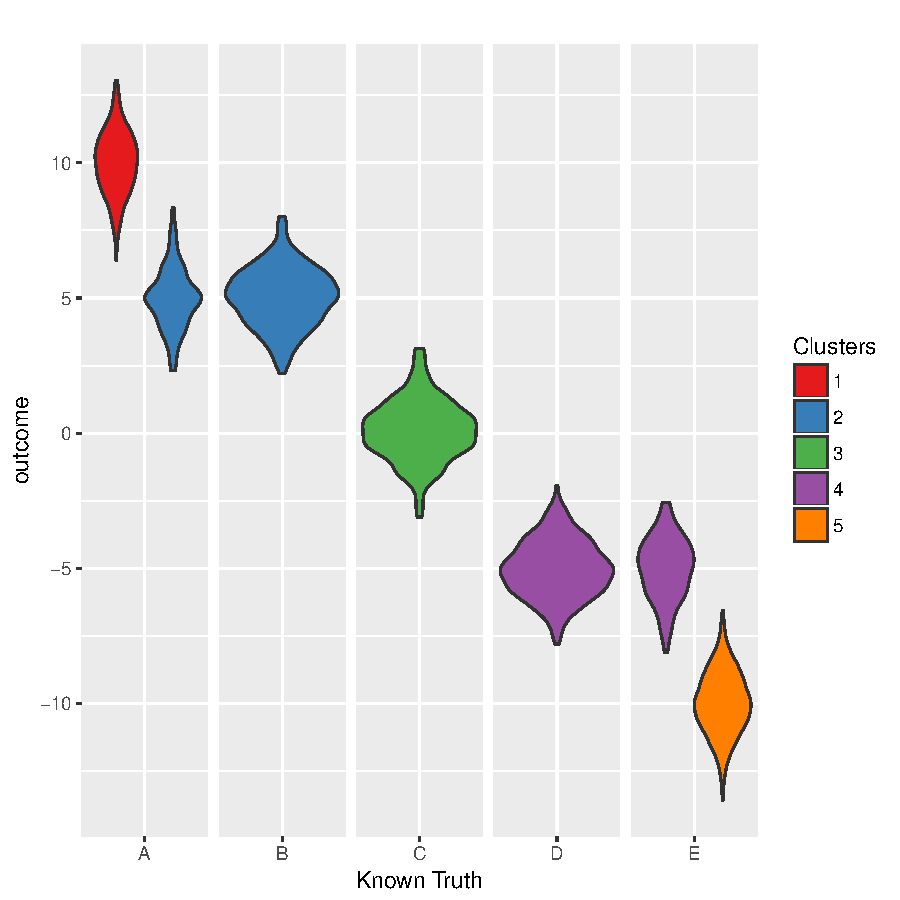
\includegraphics{Fig-test2}

We can also do this plot replacing the distribution of observed outcome with the posterior distribution of $\theta$. 

\begin{Schunk}
\begin{Sinput}
> # Construct the number of clusters file name
> nClustersFileName<-file.path(runInfoObj$directoryPath,paste(runInfoObj$fileStem,'_nClusters.txt',sep=''))
> nClustersFile<-file(nClustersFileName,open="r")
> # Construct the allocation file name
> zFileName <- file.path(runInfoObj$directoryPath,paste(runInfoObj$fileStem,'_z.txt',sep=''))
> zFile<-file(zFileName,open="r")
> # Construct the theta file name
> thetaFileName <- file.path(runInfoObj$directoryPath,paste(runInfoObj$fileStem,'_theta.txt',sep=''))
> thetaFile<-file(thetaFileName,open="r")
> firstLine<-ifelse(runInfoObj$reportBurnIn,runInfoObj$nBurn/runInfoObj$nFilter+2,1)
> lastLine<-(runInfoObj$nSweeps+ifelse(runInfoObj$reportBurnIn,runInfoObj$nBurn+1,0))/runInfoObj$nFilter
> nSamples<-lastLine-firstLine+1
> thetaByObs<-matrix(NA,ncol=runInfoObj$nSubjects,nrow=runInfoObj$nSweeps)
> for(sweep in firstLine:lastLine){
+     if(sweep==firstLine){
+       skipVal<-firstLine-1
+     }else{
+       skipVal<-0
+     }
+ 
+     currMaxNClusters<-scan(nClustersFile,what=integer(),skip=skipVal,n=1,quiet=T)
+ 
+     # Get the current allocation data for this sweep
+     currZ<-scan(zFile,what=integer(),skip=skipVal,n=runInfoObj$nSubjects+runInfoObj$nPredictSubjects,quiet=T)
+     currZ<-1+currZ
+     
+     # Get the risk data corresponding to this sweep
+     currThetaVector<-scan(thetaFile,what=double(),skip=skipVal,n=currMaxNClusters,quiet=T)
+     currTheta<-matrix(currThetaVector,ncol=1,byrow=T)
+ 
+     for (i in 1:runInfoObj$nSubjects){
+       thetaByObs[sweep,i]<-currTheta[currZ[i]]
+     }
+ }
> tmp_boxplot2<-data.frame(opt=vector(),outcome=vector(),known=vector())
> for (c in 1:max(optAlloc)){
+   for (k in names(table(known))){
+     tmp_index<-which(optAlloc==c & known==k)
+     tmp_length<-length(tmp_index)
+     if (tmp_length>1){
+       tmp_value<-apply(thetaByObs[,tmp_index],1,mean)
+       tmp_boxplot3<-data.frame(opt=rep(c,runInfoObj$nSweeps),
+                                outcome=tmp_value,known=rep(k,runInfoObj$nSweeps))
+       tmp_boxplot2<-rbind(tmp_boxplot2,tmp_boxplot3)
+     }
+     if (tmp_length==1){
+       tmp_boxplot3<-data.frame(opt=rep(c,runInfoObj$nSweeps),outcome=thetaByObs[,tmp_index],known=rep(k,runInfoObj$nSweeps))
+       tmp_boxplot2<-rbind(tmp_boxplot2,tmp_boxplot3)
+     }
+   }
+ }
> tmp_boxplot2$opt<-as.factor(tmp_boxplot2$opt)
> tmp_boxplot2$known<-as.factor(tmp_boxplot2$known)
> p <- ggplot(tmp_boxplot2, aes(x=known, y=outcome, fill=opt)) + 
+   geom_violin()+
+   labs(title="",x="Known Truth", y = "outcome") +
+   facet_grid(~known,scales='free',space='free') + 
+   guides(fill=guide_legend(title="Clusters")) +
+   theme(strip.text.x = element_blank(), strip.background = element_blank()) 
> # Use brewer color palettes
> p#+scale_fill_brewer(palette="Set1")
> # close all files
> close(zFile)
> close(nClustersFile)
> close(thetaFile)
\end{Sinput}
\end{Schunk}
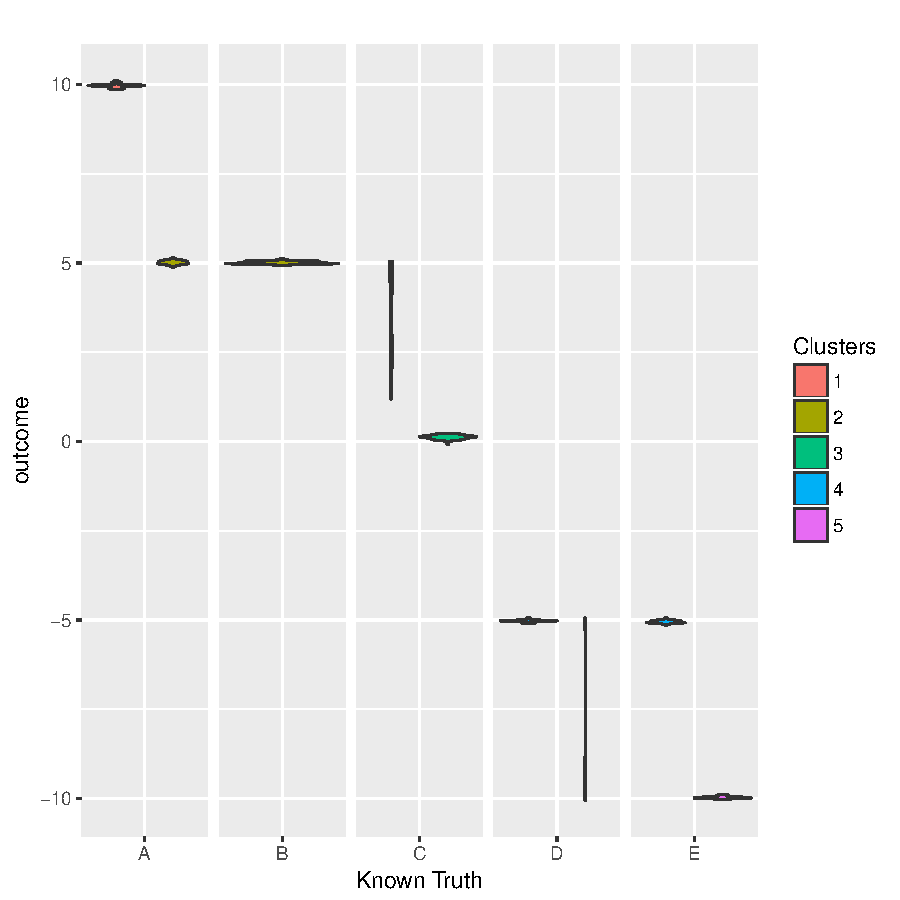
\includegraphics{Fig-test3}

Then we want to do some composite colour bars. 
\begin{Schunk}
\begin{Sinput}
> inputs <- generateSampleDataFile(clusSummaryNormalNormal())
> runInfoObj<-profRegr(yModel=inputs$yModel, 
+     xModel=inputs$xModel, nSweeps=100, nClusInit=15,
+     nBurn=300, data=inputs$inputData, output="output", 
+     covNames = inputs$covNames, 
+     seed=12345)
\end{Sinput}
\begin{Soutput}
Random number seed: 12345
Sweep: 1
\end{Soutput}
\begin{Sinput}
> dissimObj<-calcDissimilarityMatrix(runInfoObj)
\end{Sinput}
\begin{Soutput}
Stage 1:1 samples out of 100
Stage 2:1 samples out of 100
\end{Soutput}
\begin{Sinput}
> clusObj<-calcOptimalClustering(dissimObj,maxNClusters = 7)
\end{Sinput}
\begin{Soutput}
Max no of possible clusters: 7 
Trying 2 clusters
Trying 3 clusters
Trying 4 clusters
Trying 5 clusters
Trying 6 clusters
Trying 7 clusters
\end{Soutput}
\begin{Sinput}
> riskProfileObj<-calcAvgRiskAndProfile(clusObj)
\end{Sinput}
\begin{Soutput}
Processing sweep 1 of  100 
\end{Soutput}
\begin{Sinput}
> clusterOrderObj<-plotRiskProfile(riskProfileObj,"summary3.png")
\end{Sinput}
\end{Schunk}

Then we make a composite colour bar plot. 
\begin{Schunk}
\begin{Sinput}
> profile<-riskProfileObj$profile
> meanSortIndex<-clusterOrderObj
> muArray<-data.frame(covariateNumber=vector(),clusterNumber=vector(),colourPlot=vector())
> for(j in 1:runInfoObj$nCovariates){
+   # Compute the means
+   muMat<-profile[,meanSortIndex,j]
+   muMeans<-apply(muMat,2,mean)
+   muMean<-sum(muMeans*clusObj$clusterSizes)/sum(clusObj$clusterSizes)
+   muLower<-apply(muMat,2,quantile,0.05)
+   muUpper<-apply(muMat,2,quantile,0.95)
+ 
+     # Get the plot colors
+   muColor<-ifelse(muLower>rep(muMean,length(muLower)),"high",
+                 ifelse(muUpper<rep(muMean,length(muUpper)),"low","avg"))
+   muArrayNew<-data.frame(covariateNumber=rep(j,clusObj$nClusters),
+                          clusterNumber=c(1:clusObj$nClusters),
+                          colourPlot=muColor)
+   muArray<-rbind(muArray,muArrayNew)  
+ }
> ggplot(muArray, aes(x=clusterNumber, y=covariateNumber, fill=colourPlot)) +
+   geom_col(stat="identity", colour="white") 
> 
\end{Sinput}
\end{Schunk}
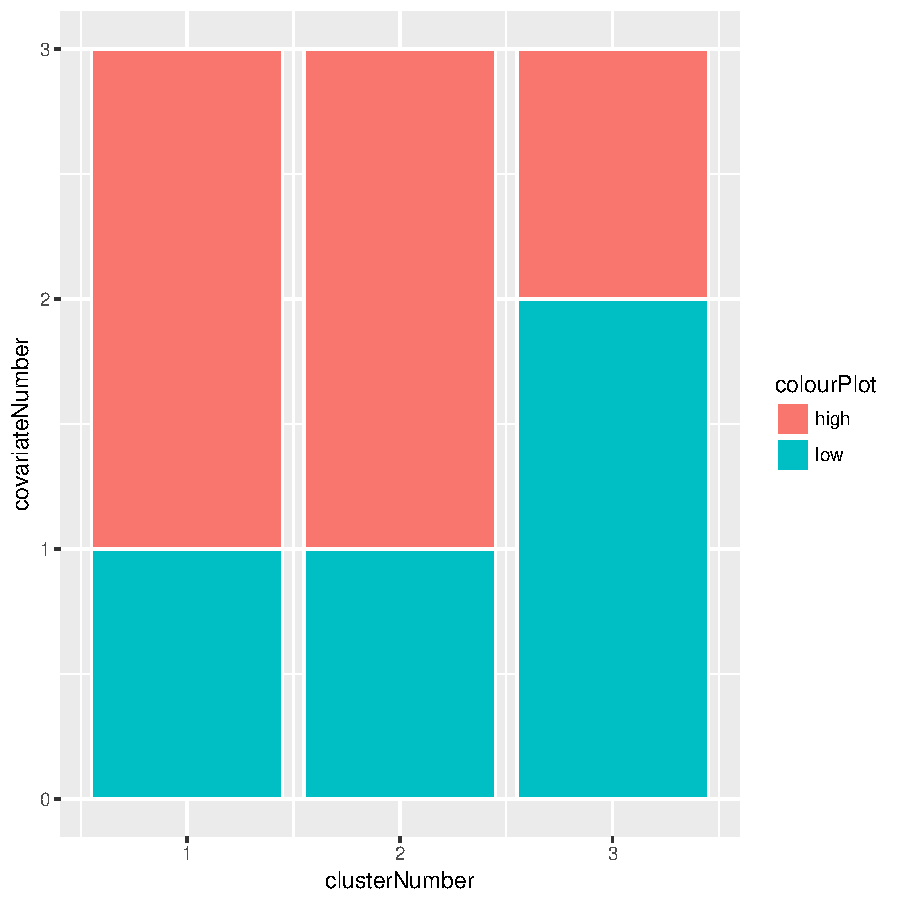
\includegraphics{Fig-test1}
%------------------------------------
\section{SessionInfo}
%-------------------------------------

This file was compiled using a computer with the following packages: 

\begin{Schunk}
\begin{Sinput}
> sessionInfo()
\end{Sinput}
\begin{Soutput}
R version 3.4.0 (2017-04-21)
Platform: x86_64-pc-linux-gnu (64-bit)
Running under: Ubuntu 16.04.2 LTS

Matrix products: default
BLAS: /usr/lib/libblas/libblas.so.3.6.0
LAPACK: /usr/lib/lapack/liblapack.so.3.6.0

locale:
 [1] LC_CTYPE=en_GB.UTF-8       LC_NUMERIC=C              
 [3] LC_TIME=en_GB.UTF-8        LC_COLLATE=en_GB.UTF-8    
 [5] LC_MONETARY=en_GB.UTF-8    LC_MESSAGES=en_GB.UTF-8   
 [7] LC_PAPER=en_GB.UTF-8       LC_NAME=C                 
 [9] LC_ADDRESS=C               LC_TELEPHONE=C            
[11] LC_MEASUREMENT=en_GB.UTF-8 LC_IDENTIFICATION=C       

attached base packages:
[1] stats     graphics  grDevices utils     datasets  methods   base     

other attached packages:
[1] ggplot2_2.2.1 PReMiuM_3.1.5

loaded via a namespace (and not attached):
 [1] Rcpp_0.12.10       digest_0.6.12      ald_1.1            MASS_7.3-47       
 [5] grid_3.4.0         plyr_1.8.4         gtable_0.2.0       magrittr_1.5      
 [9] scales_0.4.1       stringi_1.1.5      reshape2_1.4.2     lazyeval_0.2.0    
[13] labeling_0.3       RColorBrewer_1.1-2 tools_3.4.0        stringr_1.2.0     
[17] munsell_0.4.3      plotrix_3.6-4      compiler_3.4.0     colorspace_1.3-2  
[21] gamlss.dist_5.0-0  cluster_2.0.6      tibble_1.3.0      
\end{Soutput}
\end{Schunk}

\bibliographystyle{chicago}
\bibliography{biblio}
\end{document}

